
%(BEGIN_QUESTION)
% Copyright 2012, Tony R. Kuphaldt, released under the Creative Commons Attribution License (v 1.0)
% This means you may do almost anything with this work of mine, so long as you give me proper credit

Combine the equations $V = IR$, $I_{total} = I_1 + I_2$, and $V_{total} = V_1 = V_2$ for this parallel resistor circuit to solve for $I_{total}$ as a function of $V_{total}$, $R_1$, and $R_2$.  In other words, write a new equation with just $I_{total}$ on one side of the ``equals'' symbol and no variables but $V_{total}$, $R_1$, and $R_2$ on the other side:

$$\includegraphics[width=15.5cm]{i01330x01.eps}$$

$$I_{total} = f(V_{total}, R_1, R_2)$$

\underbar{file i01330}
%(END_QUESTION)





%(BEGIN_ANSWER)

$$I_{total} = {V_{total} \over R_1} + {V_{total} \over R_2}$$

Here is how we get this answer:

\begin{itemize}
\item{} First, we identify the variable we are trying to solve for; in this case it is $I_{total}$
\vskip 10pt
\item{} Next we identify which of the given equations contains this variable; in this case, it is $I_{total} = I_1 + I_2$
\vskip 10pt
\item{} Next, we look for ways to substitute $V$ and the $R$ variables for $I_1$ and $I_2$ in the first equation
\vskip 10pt
\item{} We know from Ohm's Law that $V = IR$.  Therefore, $V_1 = I_1 R_1$ and $V_2 = I_2 R_2$
\vskip 10pt
\item{} We then substitute $V_1 \over R_1$ for $I_1$, and $V_2 \over R_2$ for $I_2$ ; the result is $I_{total} = {V_1 \over R_1} + {V_2 \over R_2}$
\vskip 10pt
\item{} Using the equality $V_{total} = V_1 = V_2$ for parallel circuits, we now replace $V_1$ and $V_2$ with $V_{total}$ to get $I_{total} = {V_{total} \over R_1} + {V_{total} \over R_2}$
\end{itemize}


%(END_ANSWER)





%(BEGIN_NOTES)


%INDEX% Mathematics review: basic principles of algebra
%INDEX% Mathematics review: manipulating and combining equations to form a new equation

%(END_NOTES)


